

\documentclass[12pt]{article}
\usepackage{graphicx}
\usepackage{amsmath}
\usepackage{mathtools}
\usepackage{gensymb}

\newcommand{\mydet}[1]{\ensuremath{\begin{vmatrix}#1\end{vmatrix}}}
\providecommand{\brak}[1]{\ensuremath{\left(#1\right)}}
\providecommand{\norm}[1]{\left\lVert#1\right\rVert}
\newcommand{\solution}{\noindent \textbf{Solution: }}
\newcommand{\myvec}[1]{\ensuremath{\begin{pmatrix}#1\end{pmatrix}}}
\let\vec\mathbf

\begin{document}
\begin{center}
\textbf\large{CLASS-11\\CHAPTER-11 \\ CIRCLES}

\end{center}
\section*{Excercise 11.1}

Q2. Find the centre and radius of the given circle $(x + 5)^2 + (y – 3)^2 = 36.$

\solution
\\
Given circle equation is
\begin{align}
	(\vec{x} + 5)^2 + (\vec{y} – 3)^2 = 36 \label{1}
\end{align}
The general equation of  the circle is 
\begin{align}
	\norm{\vec{x}}^{2} + 2\vec{u}^{\top}\vec{x} + f = 0
\end{align}
Where,
\begin{align}
	\vec{u} &= -\vec{c} \text{ and } f = \norm{\vec{u}}^{2} - r^{2}\label{3}
\end{align}
by expanding \eqref{1}
\begin{align}
	\vec{x}^2+10\vec{x}+25+\vec{y}^2-6\vec{y}+9-36&=0\\
	\norm{\vec{x}}^2+2\myvec{5 & -3}\vec{x}-2&=0\label{6}
\end{align}	
by comparing \eqref{3} to \eqref{6} we get
\begin{align}
 \vec{u}&=\myvec{5\\ -3}\\
 f&=-2\\
\vec{c}&=\myvec{-5 \\ 3}\\
\norm{u}^2&=34\\
r^2&=\norm{u}^2-f\\
r^2&= 36,r=\pm6
\end{align}
radius of circle is positive so 
the centre and radius of $(x + 5)^2 + (y – 3)^2 = 36.$ is $\myvec{-5 \\ 3}$ and $6$ respectively
\begin{figure}[!h]
	\begin{center} 
	   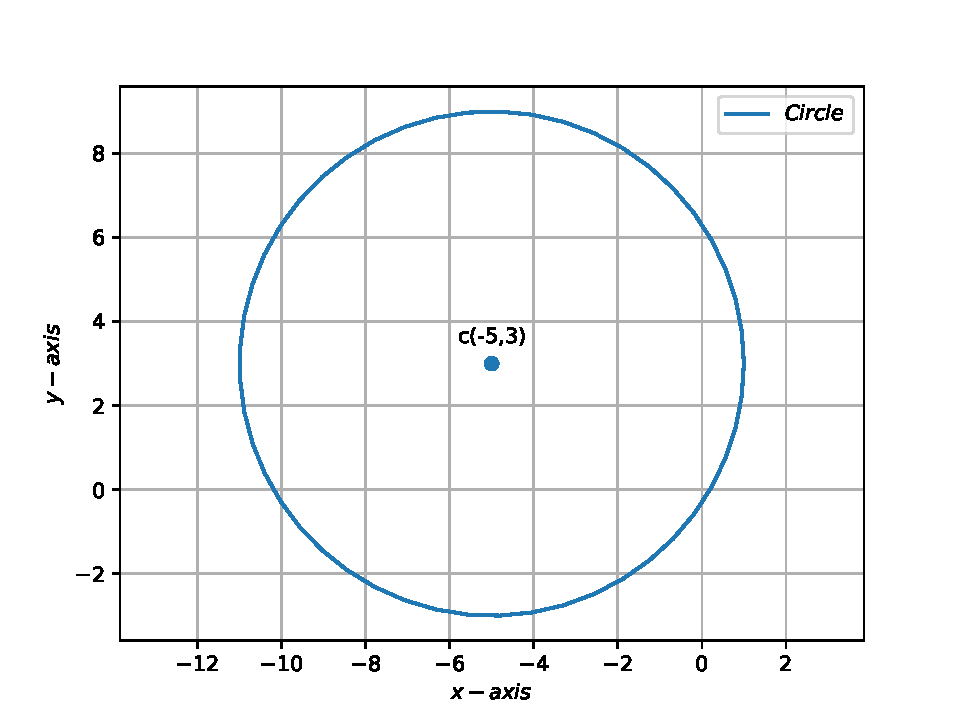
\includegraphics[width=\columnwidth]{figs/fig.pdf}
	\end{center}
\caption{}
\label{fig:Fig1}
\end{figure}

\end{document}